Filamentous microorganisms are exploited in industry for the production of a wide range of compounds of economic importance, including enzymes, organic acids, vitamins, antibiotics and, increasingly, various compounds of medicinal value \cite{archer2001,carlile2001,papagiannireview}. Historically, the fermentation of such microbes has been associated with the production of traditional oriental foods such as \emph{miso}, \emph{sh\={o}yu} (soy sauce) and \emph{tempeh}, which involves the cultivation of organisms such as \emph{Aspergillus oryzae} (\emph{k\={o}ji} mould) on solid substrates. While this practice is still common in the Far East, the submerged culture format became increasingly popular for industrial processes during the course of the 20\sp{th} century, primarily due to reduced space requirements, and is now the more commonly employed culturing method.

During cultivation in submerged fermentation, there are a range of phenotypes that can be manifested (Fig.~\ref{fig:LifeCycle}), depending on the physiology of the organism and the prevailing environmental conditions. Furthermore, there is significant evidence that the morphological form adopted by a microbe during the course of a submerged process can have a considerable influence on the level of metabolite produced, both directly and indirectly \cite{papagiannireview}. As such, developing a thorough understanding of the role of environmental variables in structural variation and the subsequent impact on productivity is a key target in the optimisation of fermentation processes.

\begin{figure}[htbp]
	\centering
	\subfloat{\label{fig:Spores}
\includegraphics[width=5cm]{../C1/Spores}}
	\hspace{1cm}
	\subfloat{\label{fig:GermSpores}
\includegraphics[width=5cm]{../C1/GermSpores}}
	\\
	\subfloat{\label{fig:Hypha}
\includegraphics[width=5cm]{../C1/Hypha}}
	\hspace{1cm}
	\subfloat{\label{fig:FreeHyphalElement}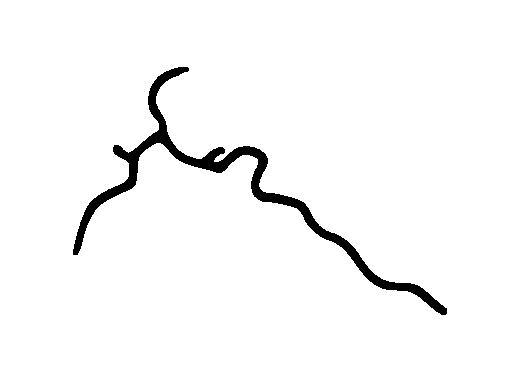
\includegraphics[width=5cm]{../C1/FreeHyphalElement}}
	\\
	\subfloat{\label{fig:MyceliumB}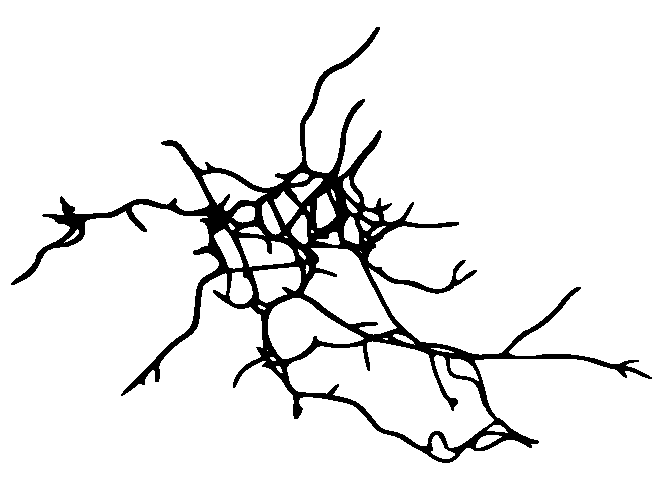
\includegraphics[width=5cm]{../C1/MyceliumB}}
	\hspace{1cm}
	\subfloat{\label{fig:Pellet}
\includegraphics[width=5cm]{../C1/Pellet}}
	\caption{Different morphological forms of filamentous microbes. Growth commences from approximately spherical spores (typically \mic{$<10$} in diameter), which, over time, produce simple branched hyphal structures (hyphal diameter is generally \mic{$<10$}). These can, in turn, develop into complex, composite architectures termed mycelia, while the agglomeration of biomass in submerged culture can result in the formation of dense, approximately spherical configurations termed \lq pellets', which may be up to several millimetres in diameter.}
	\label{fig:LifeCycle}
\end{figure}

Prior to the advent of the digital era, fungal architecture was often characterised using subjective, qualitative descriptions. However, with the proliferation of personal computers and digital cameras in the 1990's came the application of image processing techniques to the characterisation of morphology; systems capable of unsupervised, fully automated analysis of mycelial structures were soon realised \cite{packer1990,tucker1992}. However, despite this early progress, many of the image processing systems described in recent studies are not fully automated and rely on some degree of manual operation for the production of accurate data \cite{lecault2007,elsabbagh2008,anikster2005,lubbehusen2004}. Furthermore, other recent studies still lack quantitative data, reporting ambiguous, qualitative descriptions of macroscopic forms such as \lq pulpy growth', \lq smooth pellets' and \lq fluffy pellets' \cite{domingues2000,znidarsic2000}. There is therefore a pressing need for further development of automated imaging systems for this purpose.